% book example for classicthesis.sty
\documentclass[11pt,a5paper,footinclude=true,headinclude=true]{report} % KOMA-Script book
\usepackage[T1]{fontenc}                
\usepackage[linedheaders,parts,pdfspacing]{classicthesis} % ,manychapters
%\usepackage[osf]{libertine}
\usepackage{amsthm}
\usepackage{graphicx}
\usepackage[T1]{fontenc}
\newcommand{\HRule}{\rule{\linewidth}{0.5mm}}
\usepackage{float}
\RequirePackage{titletoc}


%%%%%%%%%%%%%%%%%%%%%%%%%%%%


%
\titlecontents{chapter}[1.3cm] % <-- seems to set some specific left margin
{\addvspace{3mm}}
{\makebox[0cm][r]{\large\bf\hspace{.0em}\thecontentslabel\hspace{.75cm}}}
{} %     ^^^ pretendously zero width box puts its contents in the left margin
{\hfill\makebox[-3cm]{\thecontentspage}}  % 3cm
%%
\titlecontents{section}[2cm] % <-- again this left (additional?) margin
{\addvspace{3mm}}
{\makebox[0cm][r]{\thecontentslabel\hspace{.75cm}}} % box pushed to the left
{}
{\hfill\makebox[-3cm]{\thecontentspage}}  % 3cm = twice 1.5cm
[\addvspace{0mm}]

%%%%%%%%%%%%%%%%%%%%%%%%


\begin{document}
\begin{titlepage}
    \begin{center}
        \vspace*{1cm}
        
 
        \HRule \\[0.4cm]
        {   \huge\textbf{Software Requirements and Specifications}\\[0.4cm] }
        \HRule \\[1cm]
       
        
        \vspace{0.5cm}
        \LARGE
        Thesis Subtitle
        
        \vspace{1.5cm}
        
        \textbf{The A-Team}
        
        \vfill
        
        A thesis presented for the degree of\\
        Doctor of Philosophy
        
        \vspace{0.8cm}
        
        
\includegraphics[width=0.4\textwidth]{UMASS_logo}
        
        \Large
        Department Name\\
        University Name\\
        Country\\
        Date
        
    \end{center}
\end{titlepage}
	\tableofcontents 
	
	%INTRO
\part{Introduction}
\chapter {System Overview}

The purpose of this system is to be an online tutor for students who are learning to create ER diagrams. This learning tool teaches students to build ER diagrams and allows them to submit the diagrams that they create as responses to assignment questions. The assignments are created by instructors using questions that are taken from the question bank. Each question, that is stored in 
the question bank, is created by an author and includes any correct answers and necessary feedback that correspond to it. After a student submits a diagram to be graded, he or she is either notified that diagram is correct or given feedback about the incorrectness of the diagram. This allows each student to learn from his or her mistakes. Overall, the benefits of this system are that it serves as an easier and more efficient tool for students who are learning to create ER diagrams and submitting assignments and instructors who are creating assignments and viewing student reports.  

\chapter{Stakeholders}
The stakeholders of the system involve the three defined user groups (authors, instructors and students), as well as the client, management, administrators, and developers. The administrators of the system will be involved in managing the three user groups. Administrators will give access rights to each group based on what they need to do (Authors can create questions, but instructors/students can$'$t, etc.). While the system itself has the capability to manage direct user registration the administrators have a stake in ensuring that the system is accessible to those who need it. The users all have a stake in either accessing, modifying, or creating the questions hosted within the system, and the question bank in general. The instructors who have access to the system have a stake in creating groups of questions for students and in a lesser sense creating or editing questions to their needs, and accessing reported student progress on those content clusters. Authors primarily add and edit questions in the bank and will not directly interface with student answers. Students do not create or edit questions, but answer and submit content clusters as assigned by instructors. The client and management have stakes in the system because they are responsible for providing guidance to ensure that the final product is what they want. Naturally, this leaves the developers to have a stake in the system by implementing the wants and needs of the client and management into the system.


\chapter{Scope of the Document}
This document describes the architectural layout of the online tutoring system. It includes an overview, stakeholders and a glossary to help define and describe the important system attributes. In addition, this document displays many design modules that come together to help form the architecture of the online tutoring system.  These design modules include a deployment design, which describes the technologies used for each component of the system, a  modular design, which describes the different client and server modules that are involved in transferring data, a client design, which describes all of the methods that are responsible for performing different client actions, and a server design, which describes the server$'$s role as the connection between the client and the data base.     


\chapter{Definitions}
\begin{itemize}
\item The online tutor system is the system that is being created in order to facilitate the instruction and education of constructing ER diagrams.
\item A student is a user that is accessing the online tutor system in order to learn and practice making ER diagrams.
\item The learning tool is the system that is used by a student to understand how to create ER diagrams.
An assignment is a collection of questions that the instructor selects for students to answer by a certain date.
\item Each student report, for a particular assignment, displays a unique student$'$s results to that assignment.
\item The instructor is the user who creates assignments by selecting questions from the question bank for students to answer. Also, the instructor can view the student reports for each assignment.
\item Feedback is the message that is returned to each student after he/she submits an answer. It can be composed of hints, suggestions and messages from the author.
The author is the user who creates the questions, answers and feedback. Also, the author uploads those questions, answers and feedback to the question bank for instructors to use when creating assignments.
\item Draw is the action that students or author performs to insert the shapes and words from the toolbox to the answer area of the UI. This action occurs when students are answering questions or when the author is creating answers to questions.
\item A question is created by an author (for an instructor to pull from the question bank), assigned by an instructor (in an assignment) and answered by a student (with an ER diagram).
\item  The toolbox is the area of the UI that contains all of the shapes, lines and textboxes for the user or author to drag and drop onto the draw space when drawing.
\item An answer is created by an author (with a corresponding question) and constructed by a student (in the form of an ER diagram) to respond to an assigned question. A student$'$s answer to a specific question in an assignment will be graded when that assignment is submitted.
\item NetID is the username that a user uses to log into the system.
\item Password is the password that a user uses to log into the system.
\item The question bank is the database that contains all of the questions that have been created by the author. The instructor selects questions from the question bank to create assignments for students.
\item The draw space is the area in which the answer to a question is drawn.
\item The user is the person using the online tutoring system. There are three different types of users: students, instructors and authors.
\end{itemize}  
%DIAGRAMS
\part{Diagrams}
\chapter{Deployment Design}
      In this high-level deployment diagram, we show the technologies used for each component of the system. The client will use HTML, CSS, and JS, and will be run on the user$'$s machine. This will communicated with the server, which will be built with Nodejs and will run on a Unix system. These components will use a Postgres Database in order to store all of the information of the system (user results, assignments, etc.). The database will be on the same machine as the server.
                        \begin{figure}[H]
            \centerline{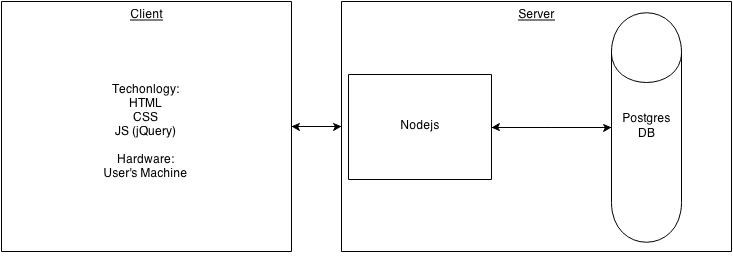
\includegraphics[height=3cm, width=10cm]{Deployment.jpg}}
            \caption{Deployment Diagram}
    \end{figure}
    
\chapter{Modular Design}
In this more detailed architecture design you can see the different modules in both the client and server sides.  The Client is made up of the Drawing Widget, Report Formatter, and Serializer while the Server is made up of the Deserializer, Dispatcher, Validator, DB Accessor and the DB.  The Drawing Widget contains everything needed for the user, author or student, to draw out either the question, answer or solution to a question that is displayed on the screen.  The Report Formatter is only used by the instructor user and takes the information that it receives from the database to compile a report on the students for the instructor to view.  The Serializer, is used for packaging and submitting the question and answer from the user to the server through http sending as a JSON.  The Deserializer is used to take what was sent from the server and undo the serialization that was used when sending information to the server.  On the Server side, the Dispatcher takes the information from the Server and packages the information to be sent to the client side of the system.  The Validator is used when a student submits an answer to a question to check the answer for correctness, and generate feedback to the student.  The DB Accessor is responsible for handling all of the requests made to send or receive information from the database.  Finally the DB is the database that contains the question bank, the student responses and assignments.    
 
                        \begin{figure}[H]
            \centerline{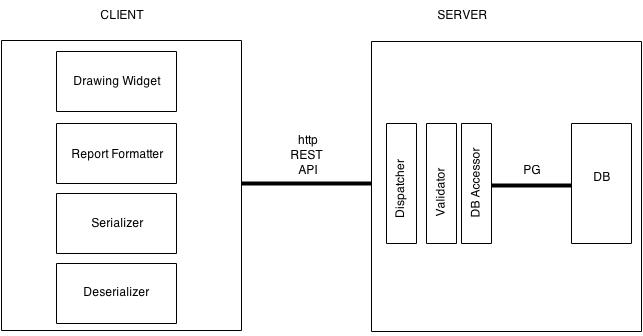
\includegraphics[height=5cm, width=10cm]{Modular.jpg}}
            \caption{Modular Diagram}
    \end{figure}
    
    \chapter{Client}
This is the diagram for the Client module. The following are the methods contained in it. openAssignment() is used by both students and instructors to open an assignment. It calls sendPageRequest() and renderPage() to render the page. createAssignment() is used by an instructor to create an assignment. openQuestion() is used by all three users, the authors, the instructors, and the students to open a question. It uses the render methods to render the page. The createQuestion() method is used by an author to create a question. drawDiagram() is used by both authors when creating the diagram and students when answering it. It uses the methods in DrawingWidget. placeEntity() to place the entities in the diagram, placeRelation() to place the relations in the diagram, and addText() to add text to the diagram. submitAnswer() is used to submit a diagram and calls sendToSerial() in DrawingWidget which uses the Serializer methods createSerialJSON() to convert the diagram into a JSON format, and sendJSON() to send this JSON to the server. openReport() is used by an instructor to view the student reports. The methods in ReportFormatter are used, collectStudentReports() retrieves the reports from the server, formatReports() formats the reports to be viewed, and render() renders the webpage.  When diagrams are sent back to the client from the server they go through the Deserializer which calls the methods, recieveJSON() when the JSON is passed back from the server and then unpackSerialJSON() to unpack the JSON back into a diagram.
  
                        \begin{figure}[H]
            \centerline{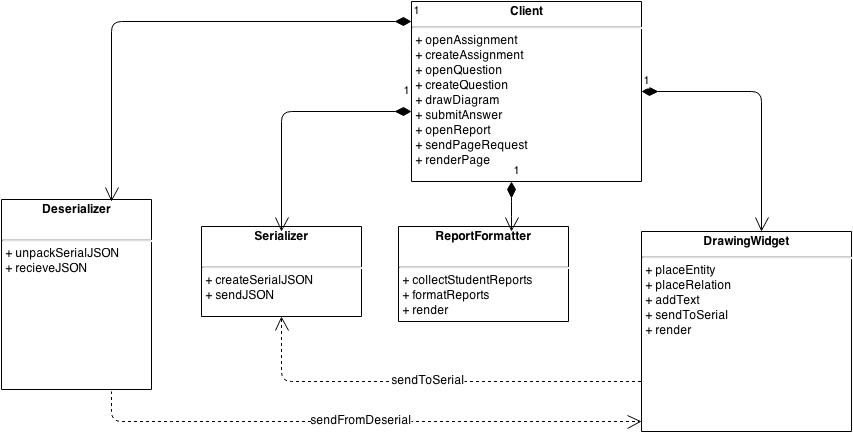
\includegraphics[height=5cm, width=10cm]{Client.jpg}}
            \caption{Client Diagram}
    \end{figure}
    
    \chapter{Server}
The server plays a huge role in our system, it is in charge of keeping connection with the Client and the database. The Dispatcher will process the question submitted by the user and request its validation with the validator. Then, the validator checks whether the question submitted by the student is actually correct or not, by going to the database accessor. Moreover, when the validator checks if a question is correct or not, it sends a customized feedback for that particular question.
The server also is able to update a particular question in the database that has been saved by the author. 

                        \begin{figure}[H]
            \centerline{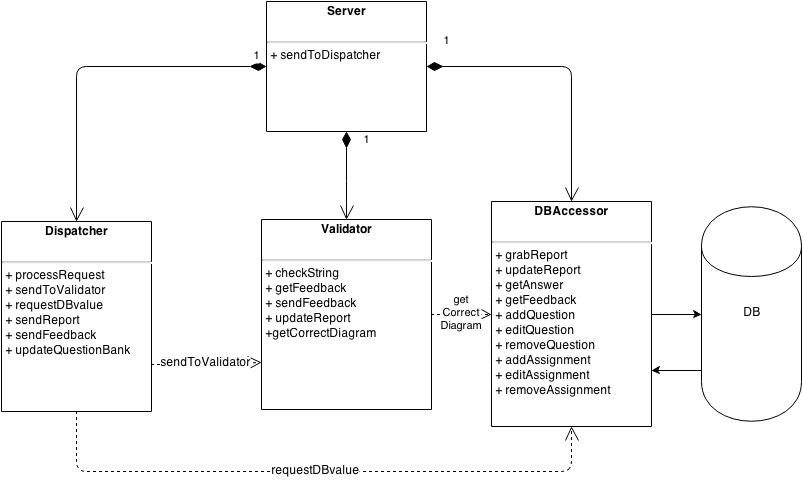
\includegraphics[height=4cm, width=10cm]{Server.jpg}}
            \caption{Server Diagram}
    \end{figure}
    






\end{document}
